\subsection{Planet Yield from the Primary Mission}
\label{sec:results_from_primary_missions}
\begin{marginfigure} %[t]
	\centering
	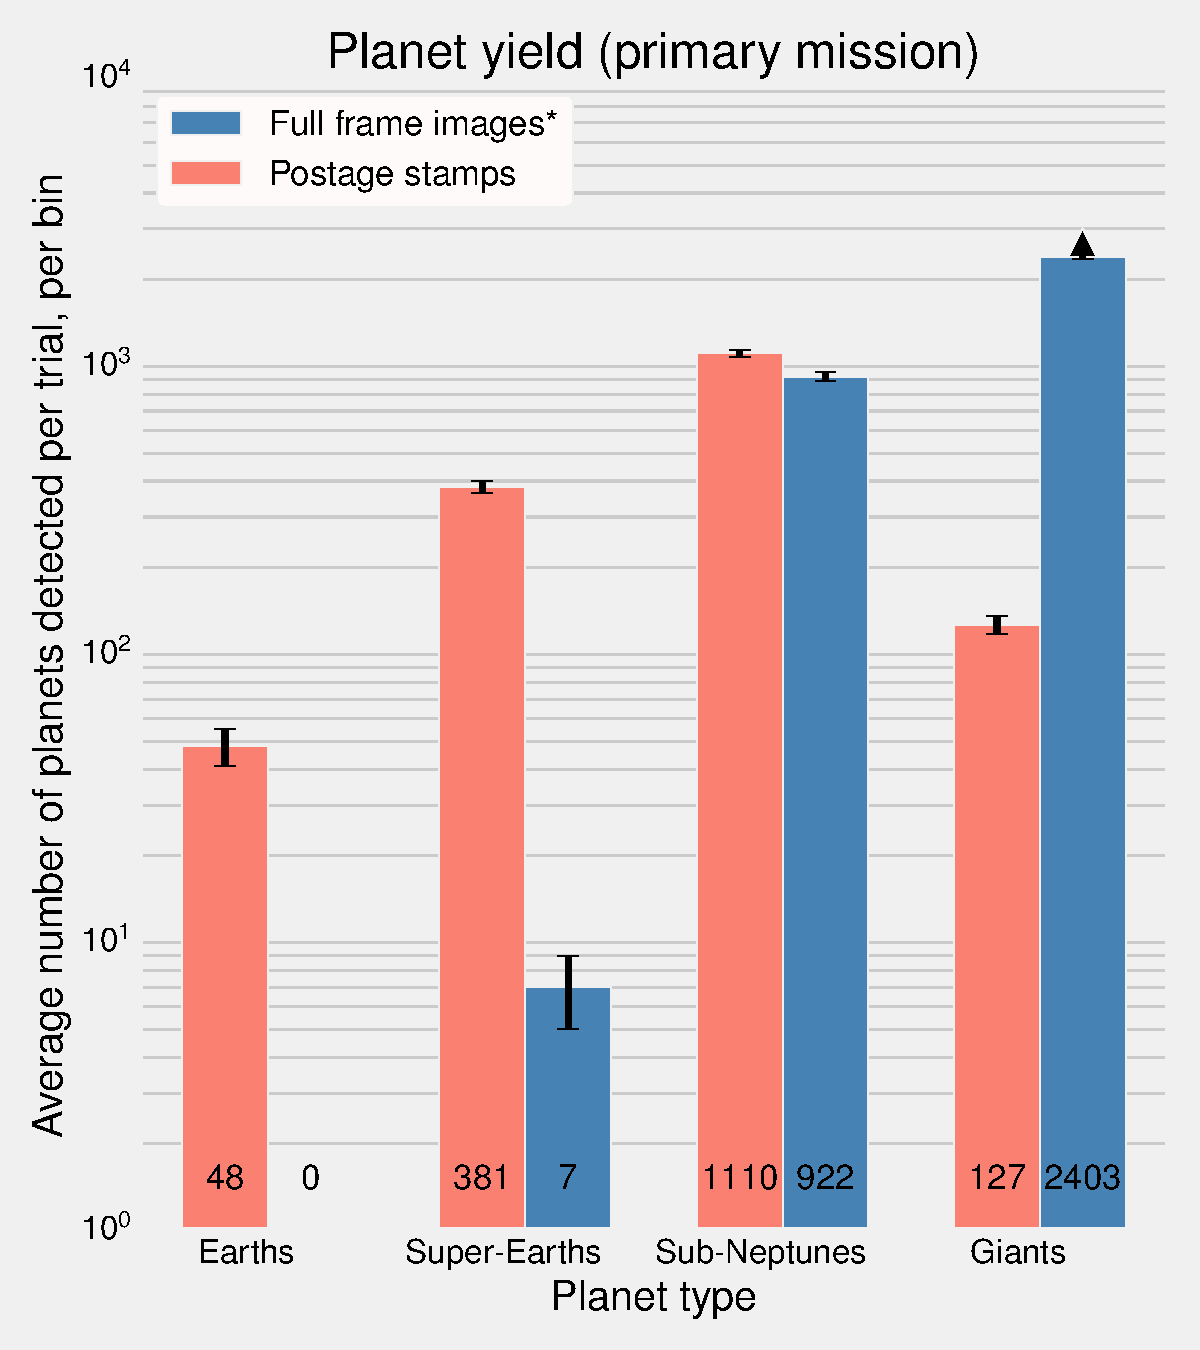
\includegraphics[width=\textwidth]{figures/160729_pm0_shemi_nhemi_nhemi_t20-pri-yield.pdf}
	\caption{Mean numbers of planets detected in \tesss Primary Mission.
	The number of Earths ($R_p < 1.25R_\oplus$), super-Earths ($1.25R_\oplus \le R_p < 2R_\oplus$), sub-Neptunes ($2R_\oplus \le R_p < 4R_\oplus$) and giants agree with the respective values quoted in \protect\citet{Sullivan_2015} to $\lesssim 50\%$. 
	%despite modifications to our target selection procedure (Sec.~\protect\ref{sec:selection_criteria}).
	Our full frame images detections are complete for $R_p < 4R_\oplus$, and 
	incomplete for giant ($R_p > 4R_\oplus$) planets, shown with a lower limit 
	(see text for discussion). 
	Error bars are from only Poisson fluctuations and do not account for systematic uncertainty.}
	\label{fig:primary_planet_yield}
\end{marginfigure}
We first examine our results for just the Primary Mission -- the first two years of \tesss observing. 
We follow with an analysis of our detected planet populations from a single Year-3 Extended Mission (Sec.~\ref{sec:results_from_nhemi_extended_mission}), and then all six of our proposed Extended Missions (Sec.~\ref{sec:results_from_all_extended_missions}).
Here we highlight commonalities and differences between~\citetalias{Sullivan_2015} and this work.

\paragraph{Detected planet yield}
The first point of consideration is the detected planet yield, shown in Fig.~\ref{fig:primary_planet_yield}.
The number of Earths, super-Earths, and sub-Neptunes we detect agrees with the numbers quoted by~\citetalias{Sullivan_2015} to within $50\%$, despite the modifications described in Sec.~\ref{sec:selection_criteria} to the target selection procedure.
Other changes to our simulation's assumptions, for instance using an as-built model of \tesss PSF informed by laboratory tests (courtesy Deborah Woods) rather than the idealized PSF described in Sec6.1 of~\citetalias{Sullivan_2015}, had minor only impact on this final result ($\lesssim 10\%$ change in yield).

A modification that did influence our lowered expected yields was a bug-fix 
in~\citetalias{Sullivan_2015}'s dilution calculation. Recall our definition of 
the dilution parameter $D$ (Eq.~\ref{eq:dilution}): placing a binary companion 
with luminosity identical to the host star into a system with a transiting 
planet that would typically transit with depth $\delta$ leads to a transit with 
`effective depth' $\delta/2$. A single missing symbol\footnote{An $\texttt{=}$ rather than 
a $\texttt{+=}$} led~\citetalias{Sullivan_2015} to under-account for this 
effect, which 
in our simulations brought about factors of $1.5\times, 1.3\times,\ 
\mathrm{and}\ 1.2\times$ fewer Earths, super-Earths, and sub-Neptunes 
respectively. This error can be noted in the published Table 6 
of~\citetalias{Sullivan_2015}, in which nearly all the dilution parameter 
values are near 1.

An additional note is that in the preparation of this report, a glaring 
discrepancy emerged between our predicted $\approx 400$ super-Earth detections 
and those shown in Fig.~18 of~\citetalias{Sullivan_2015}, which 
displays $\approx 1400$ planets. The subsequent investigation led to the discovery 
of a bug in the plotting script used to create Fig.~18. The error did not
affect any of the results described in the text, or the simulation results that were tabulated in the paper and sent electronically to interested parties.
The corrected version 
of~\citetalias{Sullivan_2015}'s Fig. 18 shows $\approx 500$ expected 
super-Earths, in much better agreement.


\begin{comment}
However, our yields from full frame images differ markedly from those quoted in Fig. 18 of~\citetalias{Sullivan_2015}.
We agree with~\citetalias{Sullivan_2015} that no Earths are detected in the full frame images.
However, we detect only $\sim$10 super-Earths by observing the $200,001\mathrm{^{st}}$ to $4,000,000\mathrm{^{th}}$ \texttt{Merit}-ranked stars at 30 minute cadence.
This is two orders of magnitude less than the $\sim$1000 super-Earth detections claimed from FFIs by~\citetalias{Sullivan_2015}.
There is also a discrepancy in FFI-detected sub-Neptunes, for which our current simulations predict that $\sim$1000 will be detected,
while~\citetalias{Sullivan_2015} predicted $\sim$2000.

We empirically verified that our full frame image detections are complete for $R < 4R_\oplus$ by enlarging the number of stars observed at 30-minute cadence and seeing that the number of detected planets with radii less than Neptune did not change.
%In this context,~\citetalias{Sullivan_2015}'s claim of detecting $1000$ super-Earths in \tesss full-frame images must be false.
We do not understand the origin of the difference between our method and~\citetalias{Sullivan_2015}'s, even after corresponding with P. Sullivan, but note that our results are in much better agreement with order-of-magnitude analytic arguments for \tesss expected planet yield.
Assuming an exponentially distributed stellar population in the galaxy and computing limiting magnitude thresholds,~\citet{winn_searchable_2013} predicted detections of $600-6000$ Neptunes, $24-300$ super-Earths, and $1-10$ Earth-sized planets, where the lower bounds correspond to planets detected with $\mathrm{SNR}>10$, and the upper bounds $\mathrm{SNR}>7$.
~\citetalias{Sullivan_2015}'s prediction of a total of $1500$ detected super-Earths is a factor of 5 larger than these analytic estimates, while
ours is in much better agreement.

Another plausibility argument that our current treatment of the FFIs
is delivering more accurate results than the code employed
by~\citetalias{Sullivan_2015} is that starting from the same input
distribution of planets, we find a more reasonable detection bias
against small planets.
One should expect that the detection bias against small planets is a steep function of radius, given that $\delta\propto R_p^2$.
\citetalias{Sullivan_2015} predicted the detection of roughly twice as many sub-Neptunes as super-Earths; our current
result has the ratio is closer to 5-to-1 which seems more realistic.
\end{comment}


\begin{comment}
  Consider the two relevant bins in the
  distribution of detected planet count \textit{vs}. planet radius.
  The $1.25R_\oplus<R_p<2R_\oplus$ bin has width $0.75R_\oplus$ and
  contains 1400 (400) detected planets according
  to~\citetalias{Sullivan_2015} (according to us).  The
  $2R_\oplus<R_p<4R_\oplus$ bin has width $2R_\oplus$ and contains 3000 (2000)
  detected planets according to~\citetalias{Sullivan_2015}
  (according to us).  The ratio of the number of detected super-Earths
  to sub-Neptunes, adjusted to the same bin width $\Delta R_p=0.75~R_\oplus$,
  is $(1400/0.75R_\oplus)/(3000/2R_\oplus)=1.25$ for \citetalias{Sullivan_2015}
  and $(400/0.75R_\oplus)/(2000/2R_\oplus)=0.53$ for our current simulations.

  The input planet occurrence distributions
  (\citetalias{Sullivan_2015}'s Fig 8) imply that the intrinsic
  population ratio in this bin is $\sim\!2$ for $T_\mathrm{eff}<4000$K
  hosts and $\sim\!1.5$ for $T_\mathrm{eff}>4000$K hosts.  Thus the
  input ratio for the number of existing super-Earths (per bin width)
  to sub-Neptunes (per bin width) across all stars is between 1.5 and
  2.
\end{comment}

% Also, Peter's data from plat10r.fits, May 4 2015, agree with my results. I never was able to find the data with his FFI numbers...

\paragraph{Properties of planets detected in Primary Mission} 

We show the population properties of planets detected in postage
stamps and full frame images during the Primary Mission in
Figs.~\ref{fig:radius_vs_period_nhemi}
and~\ref{fig:imag_vs_teff_nhemi}.  In terms of the apparent planet
radii $R_p$, orbital periods $P$, host star brightness, and host star
$T_\mathrm{eff}$, we qualitatively agree with the results
of~\citetalias{Sullivan_2015} for the planets detected
in postage stamps. 
For instance, the dearth of $P<5$ day
Neptune-radius planets in Fig.~\ref{fig:radius_vs_period_nhemi} was
observed by \textit{Kepler}~\citep{mazeh_dearth_2016}, and thus it is
present in our input occurrence rates, rather than being an
observational bias.  It was also seen by~\citetalias{Sullivan_2015}.

The differences between planets detected in postage stamps vs. in full frame images follow our expectation from our \texttt{Merit} statistic. 
Namely, Fig.~\ref{fig:imag_vs_teff_nhemi} shows that at a fixed brightness, full frame image detections tend to occur at larger stellar effective temperature (and thus stellar radius).
At a fixed host star radius, postage stamp detections occur around brighter stars.

\paragraph{Impact of earth and moon crossings on Primary Mission's detected planet yield}
During the Primary Mission, of the four cameras Camera 1 (closest to the ecliptic) suffers the most from earth and moon crossings.
As noted in Table~\ref{tab:dropped_fields}, we remove 4 of its 13 
`observing sectors' from that year.
This reduces the number of planet detections near the ecliptic, and is visible in the orange points of Fig.~\ref{fig:skymap_nhemi}.
In the Primary Mission \tess detects $\sim20$ planets with $R_p<4R_\oplus$ from both 2 minute and 30 minute data in each $24^\circ\times24^\circ$ camera field nearest to the ecliptic (where each field is observed for 2 \tess orbits).
As implemented in our simulation, Earth and Moon crossings result in fields simply not being observed, so in these cases planets orbiting stars in these fields are never detected.
Considering only the Primary Mission, we would naively expect that dropping a total of 9 fields over the two years (again, see Table~\ref{tab:dropped_fields}) would result in a loss of $\sim9\times20=180$ planets.
This agrees with what our simulations actually give: running them without accounting for Earth and Moon losses returns a mean of 2678 detected planets with $R_p<4R_\oplus$, while running them with Earth and Moon crossings gives a mean of 2482 such planets (a loss of 196 planets; $7\%$ of the $R_p<4R_\oplus$ planet yield).
% data from 160708-t50 and 160729-t20. Slightly apples to oranges because of number of trials difference, but makes the point. 
